\section{Results}

We have many parameters to take into account when we evaluate the performance of the broadcast and reduce operations. In order to make the analysis easier, we will fix some of them and vary the others.

\subsection{Broadcast}

By fixing the message size, we notice that the latency scales in a complex way with the number of processes. In fact, it is interesting to notice, as show in Figure \ref{fig:broadcast_fixed_message_size_2}, that there is a ramp up in the latency when we reach 16 processes and 32 processes. This behaviour has no clear explanation.

When we set a large message size, Figure \ref{fig:broadcast_fixed_message_size_1048576}, a substantial positive performance is observed for the binary tree algorithm. This algorithm takes advantage of the fact that the message is divided into smaller parts and sent to the processes in a binary tree fashion.

The linear algorithm, on the other hand, is the algorithm that scales worse with respect to the message size. This is not surprising as it sends the message to all processes one by one.

The mapping does not seem to have a significant impact on the performance of the broadcast operation. The performance is almost the same for all the mappings. An exception is the chain algorithm. Generally, it performs better using the map-by-core policy for the processes.

In the end, if we set the number of processes and vary the message size, we can see that the latency depends linearly on the message size. The binary tree algorithm has a better performance than the linear algorithm, as we can see in Figure \ref{fig:broadcast_fixed_processes_24}. We can see a spike in the latency in Figure \ref{fig:broadcast_fixed_processes_22} when we reach a message size of approximately 0.2 megabyte for the Binary Tree algorithm. This behaviour is not clear and needs further investigation.



\begin{figure}[h!]
    \centering
    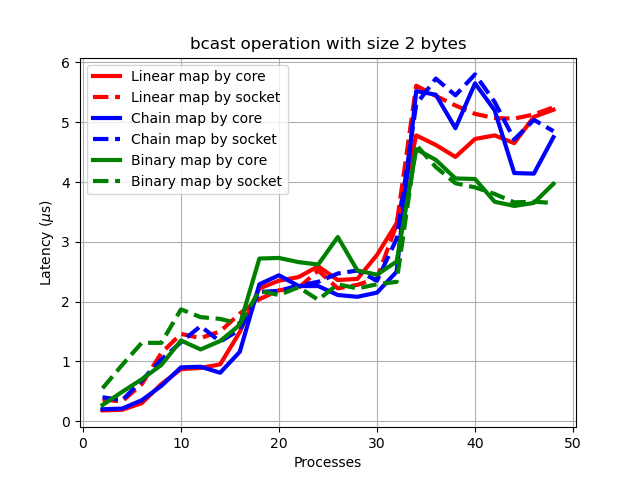
\includegraphics[width=0.7\textwidth]{../plots/bcast_fixedSize2.png}
    \caption{Broadcast 2 bytes fixed message size}
    \label{fig:broadcast_fixed_message_size_2}
\end{figure}

\begin{figure}[h!]
    \centering
    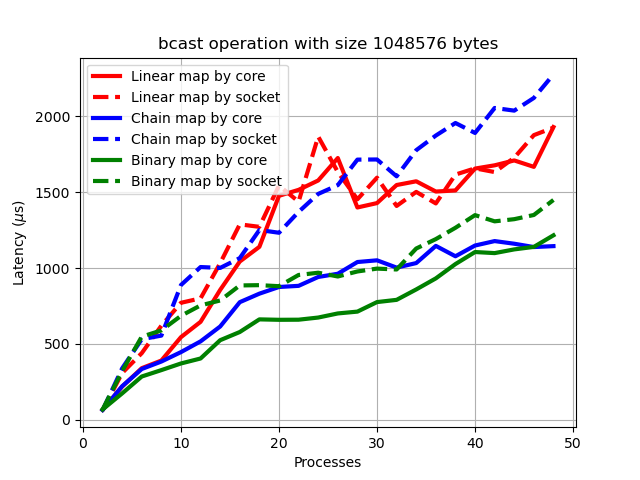
\includegraphics[width=0.7\textwidth]{../plots/bcast_fixedSize1048576.png}
    \caption{Broadcast 1 megabyte fixed message size}
    \label{fig:broadcast_fixed_message_size_1048576}
\end{figure}

\begin{figure}[h!]
    \centering
    \includegraphics[width=0.7\textwidth]{../plots/bcast_fixedProcesses2.png}
    \caption{Broadcast with 2 processes}
    \label{fig:broadcast_fixed_processes_2}
\end{figure}

\begin{figure}[h!]
    \centering
    \includegraphics[width=0.7\textwidth]{../plots/bcast_fixedProcesses24.png}
    \caption{Broadcast with 24 processes}
    \label{fig:broadcast_fixed_processes_24}
\end{figure}

\subsection{Reduce}

Let us start by setting the message size and varying the number of processes. For the reduce operation, it is interesting that the chain algorithm is the one that works worse for 2 bytes and 1024 bytes message size, as shown in Figure \ref{fig:reduce_fixed_message_size_2} and Figure \ref{fig:reduce_fixed_message_size_1024}. 
This could be explained by the fact that the chain algorithm needs to perform more operations than the other algorithms (one reduction per node)
and this is a bottleneck if the size of the message is small.

For what concernes small messages, the linear algorithm performs better than the chain algorithm.

When we set a large message size, Figure \ref{fig:reduce_fixed_message_size_1048576}, the latency scales linearly with the number of processes. Also in this case, by fixing the size of the message, the latency is proportional with the number of processes. 

As the message size increases, the mapping has no significant impact on the performance of the reduce operation performed by linear and binary algorithm. However, the chain algorithm performs significantly better using map by node policy for the processes, as depicted in Figure \ref{fig:reduce_fixed_message_size_1048576}. For large messages, the binary tree algorithm is to be preferred.

In the end, if we set the number of processes and vary the message size, we can see that the latency depends linearly on the message size. The binary tree algorithm has a better performance than the linear algorithm, as we can see in Figure \ref{fig:reduce_fixed_processes_24}. Also in this case, as expected, the tree algorithm and the chain algorithm perform better than the linear algorithm.

\begin{figure}[h!]
    \centering
    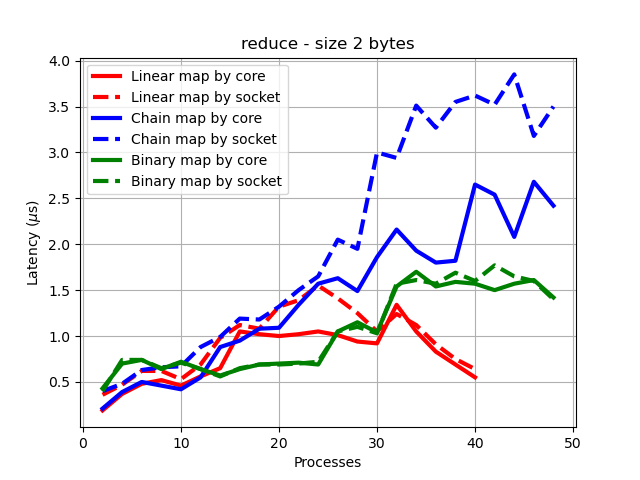
\includegraphics[width=0.7\textwidth]{../plots/reduce_fixedSize2.png}
    \caption{Reduce 2 bytes fixed message size}
    \label{fig:reduce_fixed_message_size_2}
\end{figure}

\begin{figure}[h!]
    \centering
    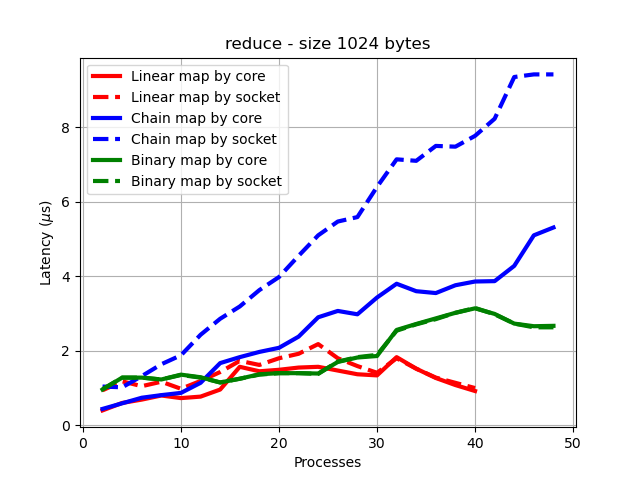
\includegraphics[width=0.7\textwidth]{../plots/reduce_fixedSize1024.png}
    \caption{Reduce 1024 bytes fixed message size}
    \label{fig:reduce_fixed_message_size_1024}
\end{figure}

\begin{figure}[h!]
    \centering
    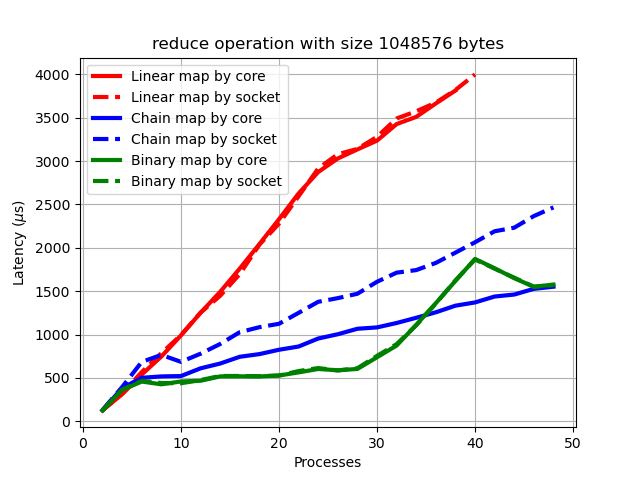
\includegraphics[width=0.7\textwidth]{../plots/reduce_fixedSize1048576.png}
    \caption{Reduce 1 megabyte fixed message size}
    \label{fig:reduce_fixed_message_size_1048576}
\end{figure}

\begin{figure}[h!]
    \centering
    \includegraphics[width=0.7\textwidth]{../plots/reduce_fixedProcesses2.png}
    \caption{Reduce with 2 processes}
    \label{fig:reduce_fixed_processes_2}
\end{figure}

\begin{figure}[h!]
    \centering
    \includegraphics[width=0.7\textwidth]{../plots/reduce_fixedProcesses24.png}
    \caption{Reduce with 24 processes}
    \label{fig:reduce_fixed_processes_24}
\end{figure}
